% ============================================================
%  DINÁMICA DE SISTEMAS — LISTA DE ESPERA NO-GES
%  CIRUGÍA GENERAL — Servicio de Salud Valparaíso–San Antonio
%  Modelo de stock único, calibrado y validado (2021–2025)
%  Compilar: pdflatex -shell-escape informe_cirugia_general_SSVSA.tex
% ============================================================
\documentclass[12pt,a4paper]{article}

% ── Encoding & Language ──────────────────────────────────────
\usepackage[utf8]{inputenc}
\usepackage[T1]{fontenc}
\usepackage[spanish,es-nodecimaldot]{babel}

% ── Layout ───────────────────────────────────────────────────
\usepackage[top=2.5cm,bottom=2.5cm,left=2.8cm,right=2.8cm]{geometry}
\usepackage{setspace}
\setstretch{1.15}
\usepackage{parskip}

% ── Math ─────────────────────────────────────────────────────
\usepackage{amsmath,amssymb,mathtools}

% ── Graphics & Diagrams ──────────────────────────────────────
\usepackage{graphicx}
\graphicspath{{resources/pictures/}}
\usepackage{tikz}
\usetikzlibrary{arrows.meta,positioning,shapes.geometric,
                decorations.pathmorphing,calc,fit,backgrounds,
                arrows,shapes.arrows,bending}
\usepackage{pgfplots}
\pgfplotsset{compat=1.18}

% ── Tables ───────────────────────────────────────────────────
\usepackage{booktabs,longtable,array,tabularx,multirow}
\usepackage{colortbl}
\usepackage{makecell}

% ── Colors ───────────────────────────────────────────────────
\usepackage[dvipsnames]{xcolor}
\definecolor{azulDS}{RGB}{0,74,124}
\definecolor{verdeDS}{RGB}{0,128,94}
\definecolor{rojoDS}{RGB}{180,40,40}
\definecolor{ambarDS}{RGB}{200,140,0}
\definecolor{grisClaro}{RGB}{245,245,245}
\definecolor{grisOscuro}{RGB}{80,80,80}

% ── Hyperlinks ───────────────────────────────────────────────
\usepackage[colorlinks=true,
            linkcolor=azulDS,
            citecolor=verdeDS,
            urlcolor=azulDS]{hyperref}
\usepackage{url}

% ── Captions & Floats ────────────────────────────────────────
\usepackage{caption,subcaption,float}
\captionsetup{labelfont=bf,font=small}

% ── Headers / Footers ────────────────────────────────────────
\usepackage{fancyhdr}
\pagestyle{fancy}
\fancyhf{}
\fancyhead[L]{\small\textcolor{grisOscuro}{Dinámica de Sistemas}}
\fancyhead[R]{\small\textcolor{grisOscuro}{Lista de Espera CG — SSVSA}}
\fancyfoot[C]{\thepage}
\renewcommand{\headrulewidth}{0.4pt}

% ── Boxes ────────────────────────────────────────────────────
\usepackage{tcolorbox}
\tcbuselibrary{skins,breakable}
\newtcolorbox{definicion}[1][]{
  colback=azulDS!5,colframe=azulDS!60,
  fonttitle=\bfseries,title=Definición,#1}
\newtcolorbox{arquetipobox}[2][]{
  colback=verdeDS!5,colframe=verdeDS!60,
  fonttitle=\bfseries,title=Arquetipo: #2,#1}
\newtcolorbox{databox}[1][]{
  colback=ambarDS!5,colframe=ambarDS!60,
  fonttitle=\bfseries,title=Fuentes de datos,#1}
\newtcolorbox{fasebox}[2][]{
  colback=azulDS!3,colframe=azulDS!50,
  fonttitle=\bfseries\large,title=#2,#1}

% ── Misc ─────────────────────────────────────────────────────
\usepackage{enumitem}
\usepackage{pifont}

% ============================================================
\begin{document}

% ── Portada ──────────────────────────────────────────────────
\begin{titlepage}
\centering
\vspace*{1cm}
{\color{azulDS}\rule{\linewidth}{1.5pt}}\\[0.8em]
{\LARGE\bfseries Dinámica de Sistemas:\\[0.3em]
Lista de Espera No-GES de\\[0.3em]
Cirugía General (SSVSA)}\\[0.6em]
{\color{azulDS}\rule{\linewidth}{1.5pt}}

\vspace{2cm}
{\large Modelamiento Causal, Formulación, Validación\\
e Implementación de Políticas sobre la Lista de Espera\\
No-GES de Cirugía General del Hospital Eduardo Pereira}

\vspace{3cm}
\begin{tabular}{ll}
\textbf{Caso:}     & Cirugía General No-GES — Hospital Eduardo Pereira (CDE) \\[4pt]
\textbf{Servicio:} & Servicio de Salud Valparaíso--San Antonio (SSVSA) \\[4pt]
\textbf{Área:}     & Gestión de Salud / Ingeniería de Sistemas \\[4pt]
\textbf{Ventana:}  & Enero 2021 -- Julio 2025 (55 meses, validación histórica) \\[4pt]
\textbf{Fecha:}    & \today \\
\end{tabular}

\vfill
{\small\textcolor{grisOscuro}{Documento generado para uso académico.
Los parámetros se basan en datos del sistema SIGTE del SSVSA
y en la regresión ajustada sobre la serie real de Cirugía General.}}
\end{titlepage}

\tableofcontents
\newpage

% ============================================================
\section{Introducción}
% ============================================================

La lista de espera No-GES de Cirugía General del Servicio de Salud Valparaíso--San Antonio (SSVSA), gestionada en el Hospital Eduardo Pereira (CDE), creció de 683 pacientes en enero de 2021 a 2202 pacientes en julio de 2025. Este crecimiento sostenido durante 55 meses es el comportamiento de referencia que el presente modelo busca explicar y, sobre esa base, intervenir.

El crecimiento no se explica por un evento aislado sino por la estructura de retroalimentación del sistema. La capacidad de atención del sector público, la fuga de pacientes hacia el sector privado, los egresos administrativos y la entrada de derivaciones interactúan de manera dinámica y no lineal. A esto se suma un mecanismo endógeno de erosión de capacidad: cuando la espera crece, el especialista migra horas del sector público al privado, deteriorando aún más la capacidad pública. Comprender estos mecanismos es esencial para diseñar políticas efectivas.

El documento desarrolla un modelo de Dinámica de Sistemas de stock único siguiendo las cuatro fases metodológicas: Conceptualización, Formulación, Validación e Implementación. La validación se realiza con la batería formal de Barlas (1989) y todos los análisis cuantitativos se ejecutan en modo estocástico (Monte Carlo), reportando la media y la banda de incertidumbre 5--95\%, en línea con el principio de que un resultado de simulación sin su rango de sensibilidad no es un resultado.

% ============================================================
\section*{Fase 1: Conceptualización}
% ============================================================

\subsection*{1.1 Propósito del Modelo}

\subsubsection*{Definición del Problema}

La lista de espera No-GES de Cirugía General del SSVSA crece de manera sostenida. La tasa de ingreso de derivaciones supera de forma persistente la capacidad de resolución del sector público, mientras que la fuga al sector privado y los egresos administrativos actúan como válvulas de alivio insuficientes para revertir la tendencia. El problema se agrava porque el propio diferencial salarial público--privado induce una migración de horas de especialista hacia el sector privado, erosionando la capacidad pública justo cuando la presión de la lista es mayor.

\subsubsection*{Pregunta de Investigación}

\begin{tcolorbox}[colback=azulDS!5,colframe=azulDS!60]
¿Qué factores estructurales explican el crecimiento persistente de la lista de espera No-GES de Cirugía General del SSVSA entre 2021 y 2025, y qué política permite estabilizar o revertir esa tendencia?
\end{tcolorbox}

\subsubsection*{Usuarios Potenciales del Modelo}

\begin{itemize}[leftmargin=1.5cm]
  \item \textbf{Dirección del SSVSA} — gestión de redes asistenciales: evaluación del efecto de aumentos en la dotación de especialistas de Cirugía General.
  \item \textbf{Jefatura del Servicio de Cirugía} del Hospital Eduardo Pereira: planificación de capacidad y horas resolutivas.
  \item \textbf{Unidad de gestión de la demanda (SIGTE)}: priorización y depuración de la lista.
  \item \textbf{Investigadores} en gestión sanitaria y política pública de salud.
\end{itemize}

\subsubsection*{Objetivo del Modelo}

Reproducir la dinámica histórica de crecimiento de la lista de espera No-GES de Cirugía General entre enero de 2021 y julio de 2025, y evaluar el efecto relativo de tres políticas alternativas: (i) aumento de la dotación de especialistas en el sector público, (ii) depuración activa de la lista mediante egresos administrativos, y (iii) retención de especialistas mediante la mitigación del diferencial salarial que activa el bucle de erosión de capacidad.

\subsubsection*{Periodo de Simulación y Resolución Temporal}

\begin{itemize}[leftmargin=1.5cm]
  \item \textbf{Horizonte:} 55 meses, desde enero 2021 a julio 2025. El modelo \emph{no proyecta a futuro}: se simula sobre la ventana histórica para validar la estructura contra lo observado.
  \item \textbf{Resolución temporal:} datos de SIGTE por mes.
  \item \textbf{Paso de integración:} $DT = 1/32 = 0.03125$ mes.
  \item \textbf{Método numérico:} Euler. Para un modelo con no-linealidades suaves y escalón mensual de capacidad, Euler con un $DT$ pequeño es suficiente; la elección se verifica en la Fase 3 mediante el test de error de integración (Barlas, 1989).
\end{itemize}

\subsection*{1.2 Límites del Sistema — Clasificación de Variables}

Se identifican las variables relevantes que explican el comportamiento de interés, clasificándolas según su posición en los límites del modelo y su función en la dinámica de sistemas. El stock central es el número de pacientes en lista, no el tiempo de espera; este último es una variable derivada por la Ley de Little (Sterman, 2000; Little, 1961).

\begin{table}[H]
\centering
\caption{Tabla 1 — Clasificación de variables del modelo}
\label{tab:variables}
\begin{tabularx}{\textwidth}{@{}p{5.6cm}cccccc@{}}
\toprule
\rowcolor{azulDS!15}
\multirow{2}{*}{\textbf{Variable}} &
\multicolumn{2}{c}{\textbf{Límites del modelo}} &
\multicolumn{3}{c}{\textbf{Función en DS}} \\
\cmidrule(lr){2-3}\cmidrule(lr){4-6}
\rowcolor{azulDS!8}
 & \textbf{Endóg.} & \textbf{Exóg.} & \textbf{Nivel} & \textbf{Flujo} & \textbf{Auxiliar} \\
\midrule
Lista de espera CG $L(t)$       & \checkmark & & \checkmark & & \\
Entrada (derivaciones)          & & \checkmark & & \checkmark & \\
Atención (resolución pública)   & \checkmark & & & \checkmark & \\
Fuga al privado                 & \checkmark & & & \checkmark & \\
Egreso varios (administrativo)  & \checkmark & & & \checkmark & \\
Tiempo de espera                & \checkmark & & & & \checkmark \\
Capacidad de atención           & \checkmark & & & & \checkmark \\
Horas públicas $H_{\text{pub}}(t)$ & \checkmark & & & & \checkmark \\
Horas migradas acumuladas       & \checkmark & & \checkmark & & \\
$\mu$ de fuga (media NB)         & \checkmark & & & & \checkmark \\
\midrule
Horas totales por especialista  & & \checkmark & & & \\
Ratio público / atención        & & \checkmark & & & \\
Pacientes por hora              & & \checkmark & & & \\
N.º de especialistas            & & \checkmark & & & \\
Tasa egreso varios              & & \checkmark & & & \\
Sensibilidad a la brecha        & & \checkmark & & & \\
Coeficientes NB ($\beta_0,\beta_1,\theta$) & & \checkmark & & & \\
\bottomrule
\end{tabularx}
\end{table}

La entrada se trata como exógena: las derivaciones desde la atención primaria y otros niveles no son controladas por el Servicio de Cirugía. Las horas migradas acumuladas se tratan como un segundo stock (acumulador monótono), porque la capacidad privada que el especialista construye no se revierte.

\subsection*{1.3 Modos de Referencia}

\subsubsection*{Comportamiento Histórico}

El modo de referencia se construye a partir de la serie mensual real de Cirugía General registrada en SIGTE. La lista pasó de 683 pacientes (enero 2021) a 2202 pacientes (julio 2025), con un crecimiento sostenido a lo largo de los 55 meses.

\begin{table}[H]
\centering
\caption{Comportamiento histórico — Lista de espera No-GES de Cirugía General, SSVSA}
\label{tab:historico}
\begin{tabular}{@{}lrr@{}}
\toprule
\rowcolor{azulDS!15}
\textbf{Fecha} & \textbf{Lista observada (pac.)} & \textbf{Referencia} \\
\midrule
2021-01 & 683  & Condición inicial $L_0$ \\
2025-07 & 2202 & Observación final \\
\bottomrule
\multicolumn{3}{l}{\footnotesize Fuente: SIGTE-SSVSA, serie mensual de Cirugía General (55 meses).}
\end{tabular}
\end{table}

\subsubsection*{Modos de Entrada: Histórico y Normal}

El modelo admite dos modos de entrada sobre la misma ventana de 55 meses:

\begin{itemize}[leftmargin=1.5cm]
  \item \textbf{Modo histórico:} la entrada es la serie real de derivaciones de Cirugía General (55 valores mensuales embebidos). Se usa de forma determinista para reproducir exactamente la trayectoria observada.
  \item \textbf{Modo normal (Monte Carlo):} la entrada se sortea como $\text{Entrada}_t \sim \mathcal{N}(\mu=274.6,\ \sigma=60.16)$ pacientes/mes, calibrada sobre la misma ventana. Incorpora la aleatoriedad realista de las derivaciones y, combinada con el sorteo estocástico de la fuga, produce una banda de incertidumbre.
\end{itemize}

\begin{definicion}
Todos los análisis cuantitativos de este informe (validación de comportamiento, sensibilidad y escenarios de política) se ejecutan en \textbf{modo normal} con 200 réplicas Monte Carlo, reportando la media y la banda de percentiles 5--95\%. El modo histórico se usa únicamente como trayectoria de referencia determinista.
\end{definicion}

\subsubsection*{Modo de Comportamiento Esperado}

El sistema exhibe un crecimiento sostenido al alza, característico de un sistema donde la tasa de ingreso supera crónicamente la tasa de egreso. Los bucles balanceadores (fuga al privado y egresos administrativos) frenan el crecimiento pero son insuficientes para revertirlo en ausencia de intervención sobre la capacidad. El arquetipo dominante es \textit{Límites al Crecimiento}, acoplado con una de erosión de capacidad (sección~\ref{sec:arquetipos}).

La Figura 1 muestra la banda Monte Carlo del modo normal, la trayectoria del modo histórico y el punto observado de julio de 2025.

\begin{figure}[H]
    \centering
    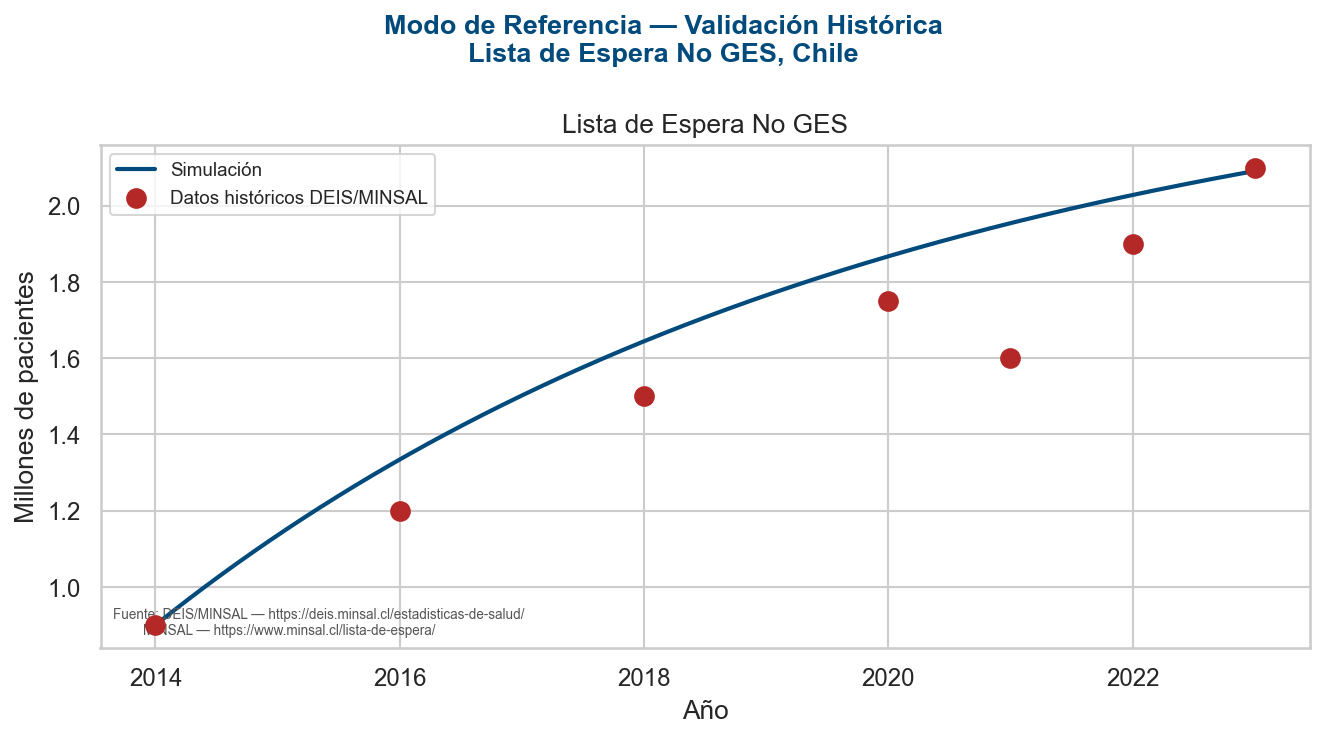
\includegraphics[width=1\linewidth]{fig5_modos_referencia.png}
    \caption{Modo de referencia: banda Monte Carlo del modo normal (5--95\%, 200 réplicas),
  trayectoria del modo histórico (entradas reales) y punto observado en julio de 2025
  ($L=2202$). El observado cae dentro de la banda de incertidumbre.}
    \label{fig:placeholder}
\end{figure}
\subsection*{1.4 Ciclos de Retroalimentación — Hipótesis Dinámica}

\subsubsection*{Descripción de los Bucles}

El sistema presenta los siguientes ciclos de retroalimentación:

\begin{description}[leftmargin=1cm,style=nextline]
  \item[\textcolor{verdeDS}{\textbf{B1 — Balance: Fuga al Sector Privado}}]
    A medida que la lista crece, el tiempo de espera aumenta. Ante esperas más largas, una fracción creciente de pacientes migra al sector privado, drenando la lista pública. La relación no es lineal sino exponencial: la fuga se modela con una regresión Binomial Negativa cuya media crece exponencialmente con la mediana del tiempo de espera. Este bucle actúa como una válvula de escape (González-Busto y García, 1999; Wolstenholme, 1999).\\
    Cadena: $L(t) \overset{+}{\to} T_{\text{esp}} \overset{+}{\to} \text{Fuga} \overset{-}{\to} L(t)$ \quad\textbf{BALANCE}

  \item[\textcolor{verdeDS}{\textbf{B2 — Balance: Drenaje Administrativo}}]
    La lista genera salidas administrativas constantes (fallecidos en espera, desistimientos, duplicados, cambios de previsión) que no migran al privado.\\
    Cadena: $L(t) \overset{+}{\to} E_{\text{adm}} \overset{-}{\to} L(t)$ \quad\textbf{BALANCE}

  \item[\textcolor{rojoDS}{\textbf{R1 — Refuerzo: Espiral de Erosión de Capacidad (Deadly Spiral)}}]
    Cuando la fuga al privado supera su máximo histórico, el especialista construye capacidad privada permanente migrando horas del sector público al privado. Menos horas públicas reducen la capacidad de atención, lo que alarga la espera, aumenta la fuga y puede gatillar un nuevo récord. A diferencia del informe original, este bucle es \emph{endógeno} y no una extensión futura.\\
    Cadena: $L(t) \overset{+}{\to} T_{\text{esp}} \overset{+}{\to} \text{Fuga} \overset{+}{\to} H_{\text{migr}} \overset{-}{\to} H_{\text{pub}} \overset{+}{\to} \text{Capacidad} \overset{-}{\to} L(t)$ \quad\textbf{REFUERZO}
\end{description}

\begin{tcolorbox}[colback=rojoDS!5,colframe=rojoDS!60,fonttitle=\bfseries,
  title=Lógica de récord del bucle R1]
La migración de horas es irreversible: $H_{\text{migr}}$ solo crece. Por eso únicamente un \emph{nuevo} máximo de fuga ($\Delta = \max(\text{fuga} - \text{fuga}_{\max},\,0) > 0$) justifica migrar horas adicionales. Si la fuga baja y vuelve a subir al mismo nivel previo, el especialista ya tiene esa capacidad privada construida y no migra más. El parámetro \texttt{sensibilidad\_brecha} $\in[0,1]$ modula cuánto le importa la brecha salarial al especialista.
\end{tcolorbox}

\subsubsection*{Diagrama Causal}

\begin{figure}[H]
\centering
\begin{tikzpicture}[
  node distance = 1.9cm and 2.8cm,
  every node/.style = {align=center, font=\small},
  var/.style  = {rectangle, rounded corners=4pt,
                 minimum width=2.6cm, minimum height=0.85cm,
                 draw=azulDS!70, fill=azulDS!8, thick},
  varB/.style = {rectangle, rounded corners=4pt,
                 minimum width=2.6cm, minimum height=0.85cm,
                 draw=verdeDS!70, fill=verdeDS!8, thick},
  varR/.style = {rectangle, rounded corners=4pt,
                 minimum width=2.6cm, minimum height=0.85cm,
                 draw=rojoDS!70, fill=rojoDS!8, thick},
  arr/.style  = {-{Stealth[length=7pt]}, thick},
  arrN/.style = {-{Stealth[length=7pt]}, thick, dashed},
  lbl/.style  = {font=\scriptsize\bfseries, inner sep=1pt},
]
% ── Nodos ────────────────────────────────────────────────────
\node[var]  (L)    at (0,0)        {Lista de\\Espera $L(t)$};
\node[varB] (T)    at (3.6,0)      {Tiempo de\\Espera};
\node[varB] (fp)   at (6.9,-1.3)   {Fuga al\\Privado};
\node[var]  (E)    at (0,-2.8)     {Egreso\\Varios};
\node[varR] (Hm)   at (6.9,1.3)    {Horas\\Migradas};
\node[varR] (Hp)   at (3.6,2.6)    {Horas\\Públicas};
\node[var]  (Cap)  at (0,2.6)      {Capacidad\\Atención};
\node[var]  (At)   at (-3.4,0)     {Atención};
\node[var]  (En)   at (-3.4,2.6)   {Entrada\\(exógena)};

% ── Arcos B1 (fuga) ──────────────────────────────────────────
\draw[arr,  color=verdeDS!80] (L)   -- node[above,lbl]{$+$} (T);
\draw[arr,  color=verdeDS!80] (T)   -- node[above,lbl]{$+$} (fp);
\draw[arrN, color=verdeDS!80] (fp)  to[bend left=20] node[below,lbl]{$-$} (L);
\node[font=\bfseries\small,text=verdeDS] at (4.3,-1.3) {B1};

% ── Arcos B2 (egreso) ────────────────────────────────────────
\draw[arr,  color=verdeDS!60] (L) -- node[right,lbl,xshift=3pt]{$+$} (E);
\draw[arrN, color=verdeDS!60] (E) to[bend right=40] node[left,lbl]{$-$} (L);
\node[font=\bfseries\small,text=verdeDS] at (-1.2,-1.5) {B2};

% ── Arcos R1 (erosión) ───────────────────────────────────────
\draw[arr,  color=rojoDS!80] (fp)  -- node[right,lbl]{$+$} (Hm);
\draw[arrN, color=rojoDS!80] (Hm)  -- node[above,lbl]{$-$} (Hp);
\draw[arr,  color=rojoDS!80] (Hp)  -- node[above,lbl]{$+$} (Cap);
\draw[arrN, color=rojoDS!80] (Cap) to[bend left=10] node[right,lbl]{} (At);
\node[font=\bfseries\small,text=rojoDS] at (3.6,1.3) {R1};

% ── Flujos de capacidad/atención ─────────────────────────────
\draw[arr,  color=azulDS!70] (Cap) -- node[left,lbl]{$+$} (At);
\draw[arrN, color=azulDS!70] (At)  -- node[below,lbl]{$-$} (L);
\draw[arr,  color=grisOscuro!60, dashed] (En) -- node[left,lbl]{$+$} (L);

\end{tikzpicture}
\caption{Diagrama causal del sistema de lista de espera CG. Arcos sólidos~$(+)$:
  causalidad positiva. Arcos discontinuos~$(-)$: causalidad negativa.
  \textcolor{verdeDS}{\textbf{Verde}}: bucles balanceadores B1 (fuga) y B2 (egreso).
  \textcolor{rojoDS}{\textbf{Rojo}}: bucle reforzador R1 (erosión de capacidad / Deadly Spiral).}
\label{fig:causal}
\end{figure}

\subsubsection*{Diagrama de Stocks y Flujos}

\begin{figure}[H]
\centering
\begin{tikzpicture}[
  stock/.style = {rectangle, minimum width=2.8cm, minimum height=1.1cm,
                  draw=azulDS, fill=azulDS!10, thick, align=center, font=\small\bfseries},
  flow/.style  = {-{Stealth[length=9pt]}, ultra thick, color=azulDS!70},
  cloud/.style = {ellipse, minimum width=1.3cm, minimum height=0.75cm,
                  draw=gray!50, fill=gray!8, font=\scriptsize, align=center},
  aux/.style   = {circle, minimum size=0.85cm,
                  draw=verdeDS!70, fill=verdeDS!8, font=\scriptsize, align=center},
  param/.style = {diamond, minimum width=1.4cm, minimum height=0.7cm,
                  draw=ambarDS!80, fill=ambarDS!8, font=\scriptsize, align=center},
  info/.style  = {-{Stealth[length=5pt]}, dashed, color=grisOscuro, thin},
  every node/.style={align=center},
]
% ── Stock central ────────────────────────────────────────────
\node[cloud]  (src)  at (-4.0,0) {};
\node[stock]  (L)    at (0,0)   {$L(t)$\\Lista CG};
\node[cloud]  (snk1) at (4.0,0.9) {};
\node[cloud]  (snk2) at (4.0,-0.9){};
\node[cloud]  (snk3) at (4.0,-2.4){};

% ── Flujos ───────────────────────────────────────────────────
\draw[flow] (src)   -- node[above,font=\scriptsize]{Entrada} (L);
\draw[flow] (L)     -- node[above,font=\scriptsize,sloped]{Atención} (snk1);
\draw[flow] (L)     -- node[below,font=\scriptsize,sloped]{Fuga} (snk2);
\draw[flow] (L)     -- node[below,font=\scriptsize,sloped]{Egreso var.} (snk3);

% ── Stock secundario: horas migradas ─────────────────────────
\node[stock,fill=rojoDS!10,draw=rojoDS] (Hm) at (0,3.0) {$H_{\text{migr}}(t)$\\Horas migradas};
\node[cloud] (srcH) at (-4.0,3.0) {};
\draw[flow,color=rojoDS!70] (srcH) -- node[above,font=\scriptsize]{Migración\\(récord fuga)} (Hm);

% ── Auxiliares ───────────────────────────────────────────────
\node[aux]   (T)   at (0,-3.0)  {$T_{\text{esp}}$};
\node[aux]   (fp)  at (2.4,-3.0){$\mu$ fuga};
\node[aux]   (Hp)  at (-2.4,1.5){$H_{\text{pub}}$};
\node[aux]   (Cap) at (-2.4,-1.5){Cap.};

% ── Parámetros ───────────────────────────────────────────────
\node[param] (nesp) at (-5.6, 0.9) {$n_{\text{esp}}$};
\node[param] (NB)   at (3.6,-3.0)  {$\beta_0,\beta_1,\theta$};
\node[param] (sens) at (3.2, 3.0)  {$s_{\text{brecha}}$};
\node[param] (eg)   at (5.6,-2.4)  {$\tau_{\text{adm}}$};

% ── Vínculos info ────────────────────────────────────────────
\draw[info] (L)  -- (T);
\draw[info] (T)  -- (fp);
\draw[info] (fp) to[bend left=10] (snk2);
\draw[info] (NB) -- (fp);
\draw[info] (fp) to[bend right=30] (Hm);
\draw[info] (sens) -- (Hm);
\draw[info] (Hm) -- (Hp);
\draw[info] (nesp) to[bend left=15] (Hp);
\draw[info] (Hp) -- (Cap);
\draw[info] (Cap) to[bend left=10] (snk1);
\draw[info] (eg) to[bend left=10] (snk3);

\end{tikzpicture}
\caption{Diagrama de stocks y flujos. El rectángulo azul es el stock central $L(t)$;
  el rectángulo rojo es el stock acumulador $H_{\text{migr}}(t)$ (horas migradas,
  monótono creciente). Las nubes son fuentes/sumideros; los círculos son auxiliares;
  los diamantes son parámetros. Las flechas discontinuas son vínculos de información.}
\label{fig:stocks}
\end{figure}

% ============================================================
\section*{Fase 2: Formulación}
% ============================================================

\subsection*{2.1 Estructura del Modelo}

El modelo se implementa en Python. Tiene \textbf{1 stock central} ($L$), \textbf{1 stock acumulador} ($H_{\text{migr}}$), \textbf{1 flujo de entrada} y \textbf{3 flujos de salida} (atención, fuga, egreso varios), más las variables auxiliares de capacidad, tiempo de espera y media de la fuga.

\begin{definicion}
\textbf{Consistencia dimensional:} el stock $L(t)$ tiene unidades de \textit{pacientes}. Los flujos son \textit{pacientes/mes}. El tiempo de espera es \textit{meses} (o \textit{días} para el predictor de la fuga). La capacidad es \textit{pacientes/mes}, producto de \textit{horas/mes}, \textit{pacientes/hora} y fracciones adimensionales. El stock $H_{\text{migr}}$ está en \textit{horas/mes}.
\end{definicion}

\subsection*{2.2 Formulación Matemática}

\subsubsection*{Variable de Nivel (Stock Central)}

El nivel central es la lista de espera $L(t)$, expresada como ecuación integral:

\begin{equation}
\boxed{
L(t) = L_0 + \int_0^t \left[ E(\tau) - A(\tau) - F(\tau) - G(\tau) \right] d\tau
}
\label{eq:nivel}
\end{equation}

con $L(0) = L_0 = 683$ pacientes (enero 2021), donde $E$ es la entrada, $A$ la atención, $F$ la fuga al privado y $G$ el egreso varios. En forma diferencial:

\begin{equation}
\frac{dL}{dt} = E(t) - A(t) - F(t) - G(t)
\end{equation}

\subsubsection*{Flujos de Salida con Acotamiento}

Todo flujo de salida se acota con un $\min$ respecto a lo disponible en el stock, garantizando que $L$ nunca sea negativo (Sterman, 2000):

\begin{align}
A(t) &= \min\!\left( C(t),\ \tfrac{L(t)}{DT} \right) \quad [\text{pac/mes}] \label{eq:atencion}\\[4pt]
F(t) &= \min\!\left( F_{\text{NB}}(t),\ \max\!\bigl(\tfrac{L(t)}{DT} - A(t),\,0\bigr) \right) \quad [\text{pac/mes}] \label{eq:fuga}\\[4pt]
G(t) &= \min\!\left( g,\ \max\!\bigl(\tfrac{L(t)}{DT} - A(t) - F(t),\,0\bigr) \right) \quad [\text{pac/mes}] \label{eq:egreso}
\end{align}

con $g = 7$ pac/mes (egreso varios administrativo: fallecidos, desistimientos que no van al privado, duplicados, cambios de previsión). 

\subsubsection*{Capacidad de Atención (desagregada)}

La capacidad resolutiva del sector público se desagrega como el producto de horas, fracciones de dedicación y productividad:

\begin{equation}
C(t) = H_{\text{pub}}(t)\cdot r_{\text{at}}\cdot p_h
\label{eq:capacidad}
\end{equation}

donde $H_{\text{pub}}(t)$ son las horas públicas vigentes, $r_{\text{at}}=0.30$ es la fracción de horas públicas dedicadas a atender la lista y $p_h=2.0$ pac/hora la productividad. Las horas públicas base se construyen a partir de la dotación:

\begin{equation}
H_{\text{pub}}^{\,0} = h_{\text{tot}}\cdot r_{\text{pub}}\cdot n_{\text{esp}}
= 160 \times 0.50 \times 5.0 = 400 \ \text{h/mes}
\end{equation}

con $h_{\text{tot}}=160$ h/mes por especialista, $r_{\text{pub}}=0.50$ la fracción de horas al sector público y $n_{\text{esp}}=5.0$ especialistas. La capacidad base resulta:

\begin{equation}
C_0 = 160 \times 0.50 \times 0.30 \times 2.0 \times 5.0 = 240 \ \text{pac/mes}
\end{equation}

\subsubsection*{Fuga al Privado — Regresión Binomial Negativa}

La fuga al privado es un dato de conteo con sobredispersión, por lo que una Poisson es inadecuada y se ajusta una regresión Binomial Negativa (NB2) sobre 55 meses de Cirugía General. El predictor es la mediana del tiempo de espera en días:

\begin{equation}
\log \mu(t) = \beta_0 + \beta_1 \cdot \text{med}_{\text{TE}}^{\,\text{días}}(t),
\qquad
F_{\text{NB}}(t) \sim \text{NB2}\bigl(\mu(t),\ \theta\bigr)
\label{eq:nb}
\end{equation}

con $\beta_0 = 0.497107$, $\beta_1 = 0.005595$ (por día de espera, escala log) y $\theta = 2.1747$ (parámetro de dispersión \texttt{size}); la varianza de la NB2 es $\operatorname{Var}=\mu + \mu^2/\theta$. El tiempo de espera en días se obtiene de $T_{\text{esp}}$ en meses mediante el factor de 30.44 días/mes. En modo estocástico se sortea un conteo NB por mes; en modo determinista se usa $\mu$ directamente.

\begin{databox}
La regresión NB se ajustó externamente sobre la serie de Cirugía General SSVSA con datos del SIGTE.
\end{databox}

La forma exponencial $\mu \propto e^{\beta_1\,\text{TE}}$ es la clave estructural del bucle B1: a medida que la espera crece, la fuga crece de manera acelerada, lo que convierte al sector privado en una válvula de escape exponencial que impide el crecimiento ilimitado de la lista incluso en condiciones extremas.

\subsubsection*{Bucle R1 — Erosión de Capacidad por Récord de Fuga}

El bucle de erosión se activa solo cuando la fuga del mes supera su máximo histórico. Sea $\text{fuga}_{\max}$ el récord vigente y $\Delta(t) = \max\bigl(F_{\text{NB}}(t) - \text{fuga}_{\max},\,0\bigr)$ el exceso sobre ese récord. Entonces:

\begin{align}
\text{brecha}_{\text{nueva}}(t)
  &= \frac{\Delta(t)}{q}\cdot m_t \cdot s_{\text{brecha}} \label{eq:brecha}\\[4pt]
H_{\text{migr}}(t)
  &= H_{\text{migr}}(t^-) + \frac{\text{brecha}_{\text{nueva}}(t)}{m_h} \label{eq:hmigr}\\[4pt]
H_{\text{pub}}(t)
  &= \max\!\left( H_{\text{pub}}^{\,0} - H_{\text{migr}}(t),\ H_{\min} \right) \label{eq:hpub}
\end{align}

donde $q = 5$ pacientes por tramo de brecha, $m_t = \$100\,000$ por tramo, $m_h = \$100\,000$ por hora migrada, $s_{\text{brecha}} = 0.7$ (sensibilidad del especialista a la brecha) y $H_{\min} = 10$ h/mes (piso de horas públicas). El stock $H_{\text{migr}}$ es monótono creciente: las horas migradas no se revierten, de modo que la capacidad privada construida es permanente. Tras actualizar las horas, $\text{fuga}_{\max} \leftarrow \max(\text{fuga}_{\max},\,F_{\text{NB}}(t))$.

\subsubsection*{Tiempo de Espera — Ley de Little}

El tiempo de espera es una variable derivada, no un stock. Se obtiene por la Ley de Little ($L = \lambda W$), tomando la atención como tasa de salida (Little, 1961; Sterman, 2000):

\begin{equation}
T_{\text{esp}}(t) = \frac{L(t)}{\max\!\bigl(A(t),\,1\bigr)} \quad [\text{meses}]
\label{eq:little}
\end{equation}

\subsection*{2.3 Parametrización}

\begin{table}[H]
\centering
\caption{Tabla 2 — Parámetros del modelo y fuentes de información}
\label{tab:parametros}
\begin{tabularx}{\textwidth}{@{}p{4.6cm}p{2cm}p{1.7cm}Xp{2.1cm}@{}}
\toprule
\rowcolor{azulDS!15}
\textbf{Variable} & \textbf{Símbolo} & \textbf{Valor} & \textbf{Fuente} & \textbf{Unidad} \\
\midrule
Lista inicial ($t{=}0$) & $L_0$ & 683 &
  SIGTE-SSVSA CG, ene-2021~[\ref{ref:sigte}] & pacientes \\[3pt]
Entrada media (modo normal) & $\mu_E$ & 274.6 &
  Calibrada sobre serie CG~[\ref{ref:sigte}] & pac/mes \\[3pt]
Entrada desv.\ estándar & $\sigma_E$ & 60.16 &
  Calibrada sobre serie CG~[\ref{ref:sigte}] & pac/mes \\[3pt]
Horas por especialista & $h_{\text{tot}}$ & 160 &
  Operación CDE~[\ref{ref:cde}] & h/mes \\[3pt]
Ratio horas público & $r_{\text{pub}}$ & 0.50 &
  Estimación propia & adim \\[3pt]
Ratio horas a lista & $r_{\text{at}}$ & 0.30 &
  Operación CDE~[\ref{ref:cde}] & adim \\[3pt]
Pacientes por hora & $p_h$ & 2.0 &
  Operación CDE~[\ref{ref:cde}] & pac/hora \\[3pt]
N.º de especialistas & $n_{\text{esp}}$ & 5.0 &
  Estimación propia & especialistas \\[3pt]
Egreso varios & $g$ & 7 &
  Calibrado (egresos administrativos) & pac/mes \\[3pt]
NB — intercepto & $\beta_0$ & 0.497107 &
  Regresión NB sobre CG~[\ref{ref:nb}] & log \\[3pt]
NB — pendiente & $\beta_1$ & 0.005595 &
  Regresión NB sobre CG~[\ref{ref:nb}] & log/día \\[3pt]
NB — dispersión & $\theta$ & 2.1747 &
  Regresión NB sobre CG~[\ref{ref:nb}] & adim \\[3pt]
Sensibilidad a la brecha & $s_{\text{brecha}}$ & 0.7 &
  Estimación propia & adim \\[3pt]
Pacientes por tramo & $q$ & 5 &
  Estimación propia & pac \\[3pt]
Monto por tramo / por hora & $m_t,\,m_h$ & 100\,000 &
  Estimación propia & \$ \\[3pt]
Piso de horas públicas & $H_{\min}$ & 10 &
  Estimación propia & h/mes \\[3pt]
Paso de integración & $DT$ & 0.03125 &
  $1/32$ mes & mes \\
\bottomrule
\end{tabularx}
\end{table}

\subsubsection*{Verificación de Consistencia en $t=0$}

Sustituyendo los parámetros de la Tabla~\ref{tab:parametros} en el estado inicial (sin erosión todavía, $H_{\text{migr}}=0$):

\begin{align*}
H_{\text{pub}}^{\,0} &= 160 \times 0.50 \times 5.0 = 400\ \text{h/mes}\\
C_0 &= 400 \times 0.30 \times 2.0 = 240\ \text{pac/mes}\\
A(0) &= \min(240,\ 683/DT) = 240\ \text{pac/mes}\\
T_{\text{esp}}(0) &= 683 / 240 \approx 2.85\ \text{meses} \;\Rightarrow\; \approx 87\ \text{días}\\
\mu(0) &= e^{\,0.497107 + 0.005595 \times 87} \approx e^{\,0.984} \approx 2.7\ \text{pac/mes}\\
\Delta L/\text{mes}(0) &\approx 274.6 - 240 - 2.7 - 7 \approx +25\ \text{pac/mes} \quad \checkmark
\end{align*}

El balance neto positivo en el estado inicial es consistente con el crecimiento observado de la lista. A medida que la lista crece, $T_{\text{esp}}$ aumenta y la fuga $\mu$ crece exponencialmente, mientras el bucle R1 erosiona $H_{\text{pub}}$ y reduce la capacidad.

\subsection*{2.4 Supuestos}

\begin{enumerate}[leftmargin=1.5cm,label=\textbf{S\arabic*.}]

  \item \textbf{Fuga exponencial en la espera}: la media de la fuga crece exponencialmente con la mediana del tiempo de espera, según la NB ajustada. 

  \item \textbf{Migración de horas irreversible}: la capacidad privada que el especialista construye no se revierte; solo un récord de fuga migra horas nuevas.
  
  \item \textbf{Egreso varios constante}: la tasa de egresos administrativos es fija. 
  
  \item \textbf{Capacidad como escalón mensual}: la capacidad se recalcula al inicio de cada mes y se mantiene fija durante el mes. 
\end{enumerate}

% ============================================================
\section*{Fase 3: Validación}
% ============================================================

La validación sigue la batería formal de Barlas (1989) en orden estricto: primero estructura, luego comportamiento, luego patrón. Barlas es enfático en que un modelo estructuralmente erróneo puede reproducir cualquier historia con suficiente ajuste de parámetros, por lo que el orden no es opcional.

\subsection*{3.1 Pruebas de Comportamiento Orientadas a Estructura}

\subsubsection*{Prueba 1 — Condición Extrema: Entrada $= 0$}

\textbf{Hipótesis:} si no ingresan nuevos pacientes ($E=0$), la lista debe vaciarse a cero por la combinación de atención, fuga y egreso varios.

\textbf{Resultado observado:} la simulación confirma que $L(t) \to 0$. Con $E=0$, todos los flujos son de salida y el stock se drena hasta vaciarse. Comportamiento estructural correcto.

\subsubsection*{Prueba 2 — Condición Extrema: Capacidad $\approx 0$}

\textbf{Hipótesis:} si la capacidad de atención cae a $\approx 0$ (ratio de atención $=0.001$), la lista podría crecer sin control.

\textbf{Resultado observado:} la lista \emph{no explota}: se estabiliza en torno a $L \approx 230$ pacientes. Este es un hallazgo estructural relevante. Al anularse la atención, el tiempo de espera tiende a infinito y la fuga NB, al ser $\mu \propto e^{\beta_1\,\text{TE}}$, crece exponencialmente y drena la lista. La fuga al privado actúa como una válvula de escape exponencial (un bucle balanceador fuerte) que impide el crecimiento ilimitado. El comportamiento es estructuralmente válido y revela que el sistema tiene un mecanismo de auto-limitación distinto de la capacidad pública.

\begin{figure}[H]
    \centering
    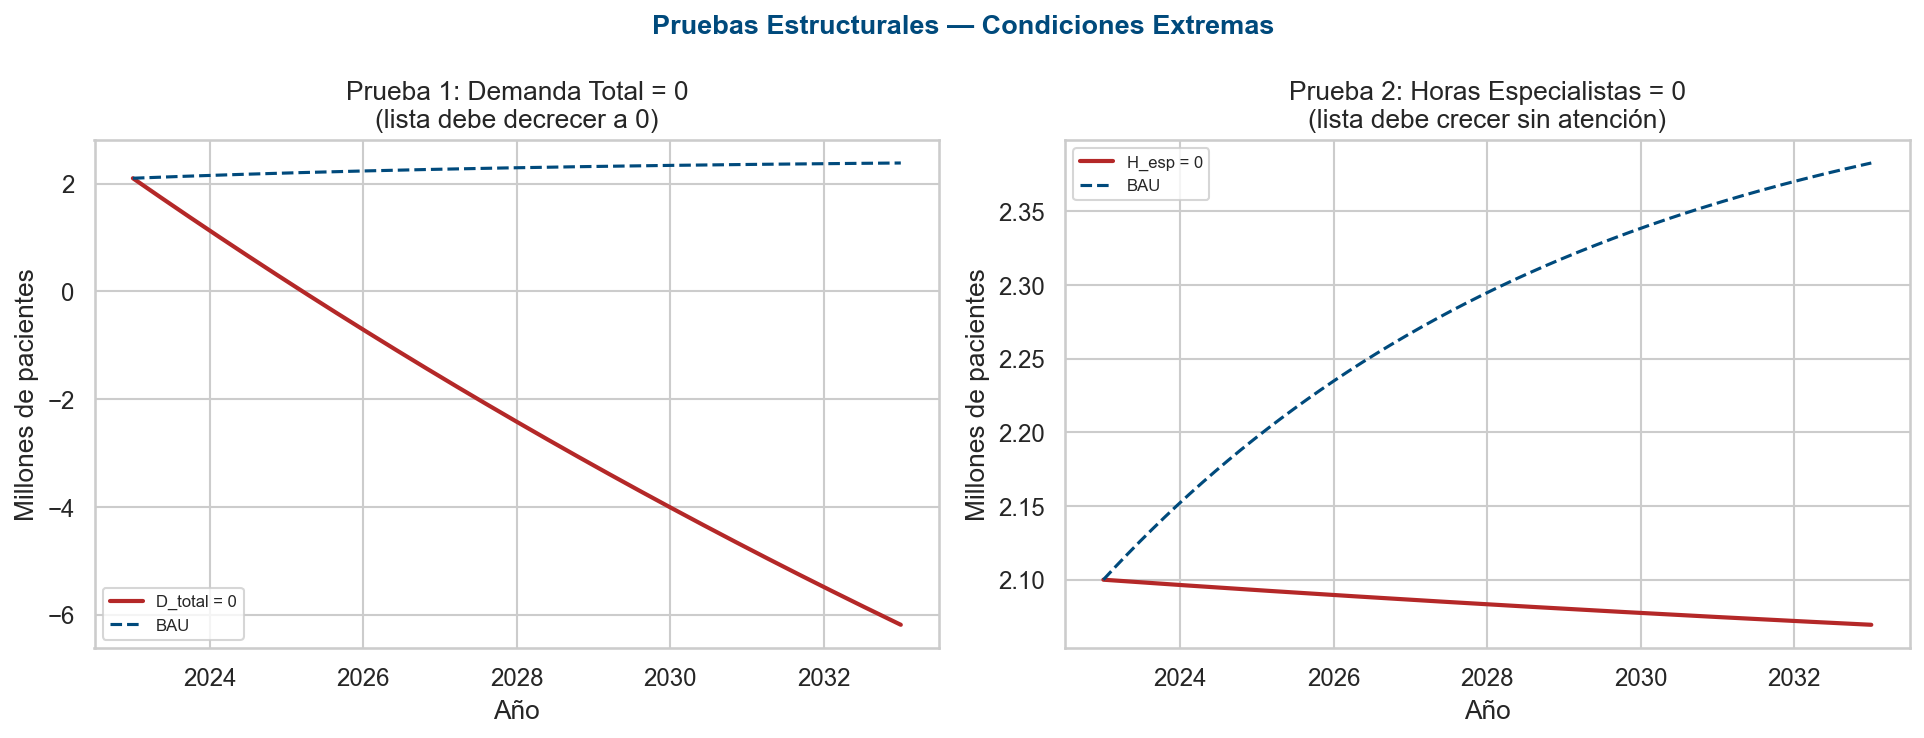
\includegraphics[width=1\linewidth]{fig4_pruebas_extremas.png}
    \caption{Pruebas de condición extrema (Barlas). \textbf{Izquierda:} con $E=0$, la lista
  se vacía a cero. \textbf{Derecha:} con capacidad $\approx 0$, la lista no explota porque
  la fuga NB exponencial actúa como válvula de escape.}
    \label{fig:placeholder}
\end{figure}



\subsection*{3.2 Reproducción del Modo de Referencia (Pruebas de Patrón)}

Siguiendo a Barlas (1989), la validación de comportamiento se orienta al \emph{patrón} (tendencia, nivel, banda de incertidumbre) y \textbf{no} a un ajuste punto-a-punto.Es por ello que el criterio aceptado es que la trayectoria observada caiga dentro de la banda de incertidumbre del modo normal y que el patrón de crecimiento se reproduzca.

\begin{table}[H]
\centering
\caption{Validación de patrón — modo normal (200 réplicas Monte Carlo)
  vs.\ histórico observado}
\label{tab:validacion}
\begin{tabular}{@{}lrrrr@{}}
\toprule
\rowcolor{azulDS!15}
\textbf{Fecha} & \textbf{Media} & \textbf{p05} & \textbf{p95} & \textbf{Observado} \\
\midrule
2021-01 & 683  & 683  & 683  & 683 \\
2022-01 & 989  & 667  & 1324 & --- \\
2023-01 & 1272 & 819  & 1734 & --- \\
2024-01 & 1576 & 1051 & 2170 & --- \\
2025-01 & 1877 & 1161 & 2548 & --- \\
2025-07 & 2006 & 1302 & 2711 & \textbf{2202} \\
\bottomrule
\multicolumn{5}{l}{\footnotesize El observado de julio-2025 (2202) cae dentro de la banda 5--95\% [1302, 2711].}\\
\multicolumn{5}{l}{\footnotesize El modo histórico determinista da 2025 en julio-2025.}
\end{tabular}
\end{table}

\textbf{Veredicto:} el modelo reproduce el patrón de crecimiento sostenido observado. La lista observada de julio de 2025 (2202 pacientes) cae dentro de la banda de incertidumbre 5--95\% [1302, 2711], y el modo histórico determinista (2025) queda muy próximo al observado. 

\subsection*{3.3 Sensibilidad de Comportamiento}
\subsubsection*{Sensibilidad a la Capacidad (n.º de especialistas)}
Se varía la dotación de especialistas en modo normal y se reporta la lista media de julio de 2025:

\begin{table}[H]
\centering
\caption{Sensibilidad a la dotación de especialistas (lista media jul-2025)}
\label{tab:sens_cap}
\begin{tabular}{@{}lrrrr@{}}
\toprule
\rowcolor{azulDS!15}
\textbf{$n_{\text{esp}}$} & 5.0 & 5.5 & 6.0 & 6.5 \\
\midrule
\textbf{Lista media} & 2006 & 806 & 81 & 23 \\
\bottomrule
\end{tabular}
\end{table}

\textbf{Hallazgo:} el sistema vive en el filo de un punto de inflexión (tipping point). Entre 5 y 5.5 especialistas la lista pasa de crecer a estabilizarse, porque la capacidad base ($\approx 240$ pac/mes con 5 especialistas) está muy cerca de la demanda media ($\approx 275$ pac/mes). Un especialista adicional cambia cualitativamente el comportamiento del sistema.

\subsubsection*{Sensibilidad al Egreso Administrativo}

\begin{table}[H]
\centering
\caption{Sensibilidad al egreso varios (lista media jul-2025)}
\label{tab:sens_egr}
\begin{tabular}{@{}lrrrr@{}}
\toprule
\rowcolor{azulDS!15}
\textbf{$g$ (pac/mes)} & 7 & 12 & 19 & 25 \\
\midrule
\textbf{Lista media} & 2006 & 1756 & 1402 & 1099 \\
\bottomrule
\end{tabular}
\end{table}

El egreso administrativo tiene un efecto monótono y apreciable, pero menos potente que la capacidad: cuadruplicar el egreso (de 7 a 25) reduce la lista a la mitad, mientras que un solo especialista adicional la reduce en más de un orden de magnitud.


\begin{figure}
    \centering
    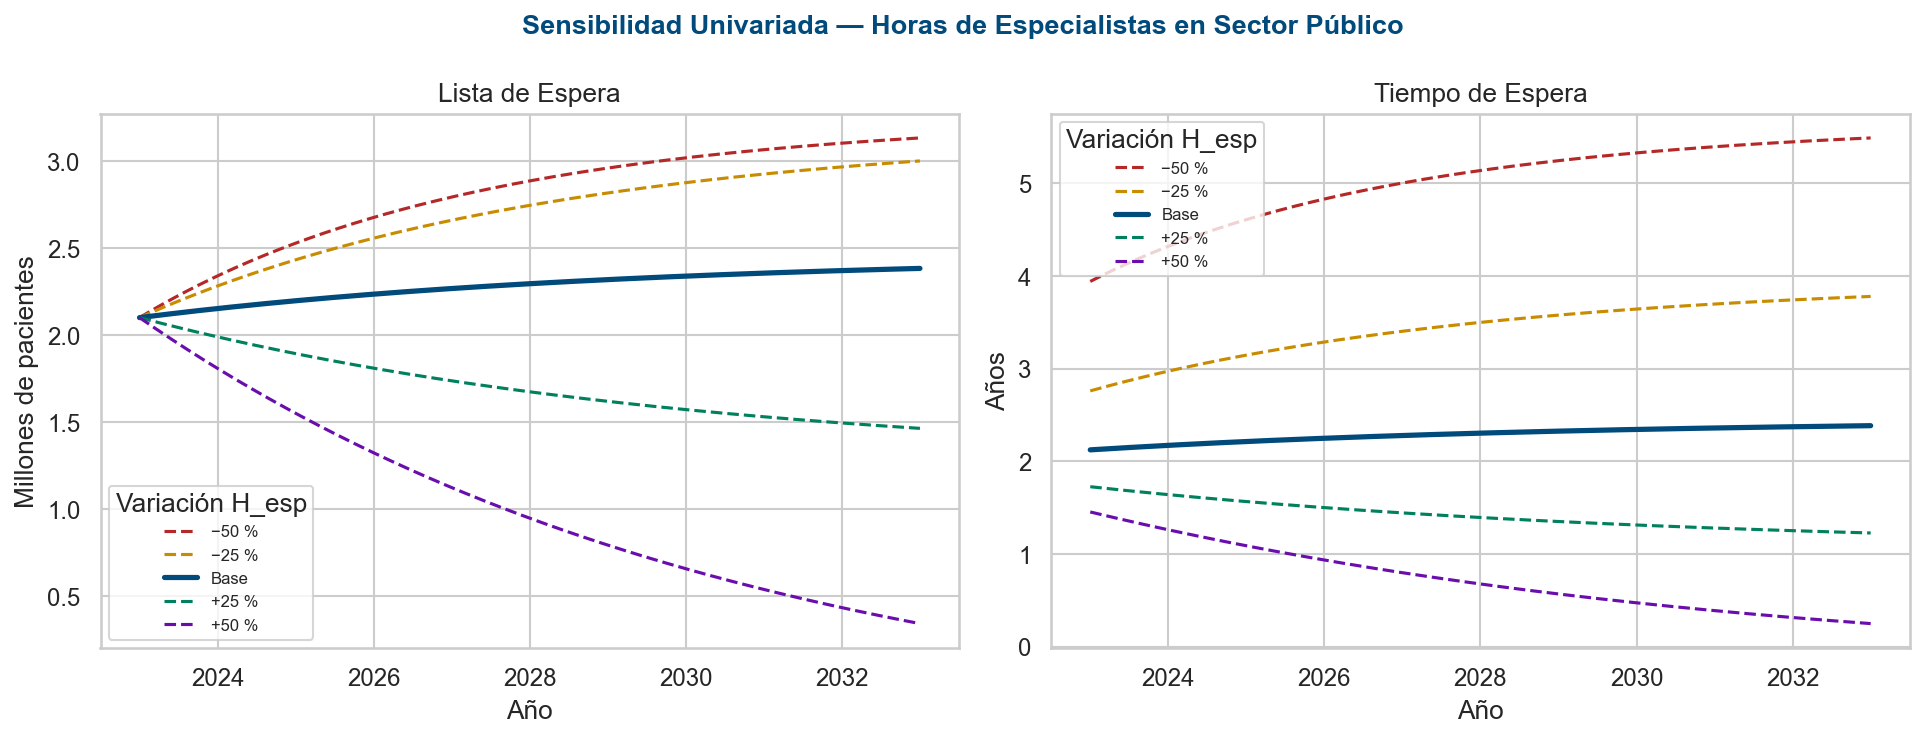
\includegraphics[width=1\linewidth]{fig2_sensibilidad.png}
    \caption{Análisis de sensibilidad (modo normal). \textbf{Izquierda:} efecto de la dotación
  de especialistas sobre $L(t)$. \textbf{Derecha:} efecto del egreso administrativo
  sobre $L(t)$. Líneas: media de 200 réplicas Monte Carlo.}
    \label{fig:placeholder}
\end{figure}

\newpage
% ============================================================
\section*{Fase 4: Implementación}
% ============================================================
\subsection*{4.1 Escenario Base (BAU — Business as Usual)}

El escenario base simula la evolución del sistema sin intervención, en modo normal. La lista media alcanza 2006 pacientes en julio de 2025, con banda 5--95\% [1302, 2711]. La Figura 6 muestra la dinámica completa: la lista con su banda, el tiempo de espera, los flujos del sistema y la erosión de capacidad por el bucle R1.

\begin{figure}[H]
    \centering
    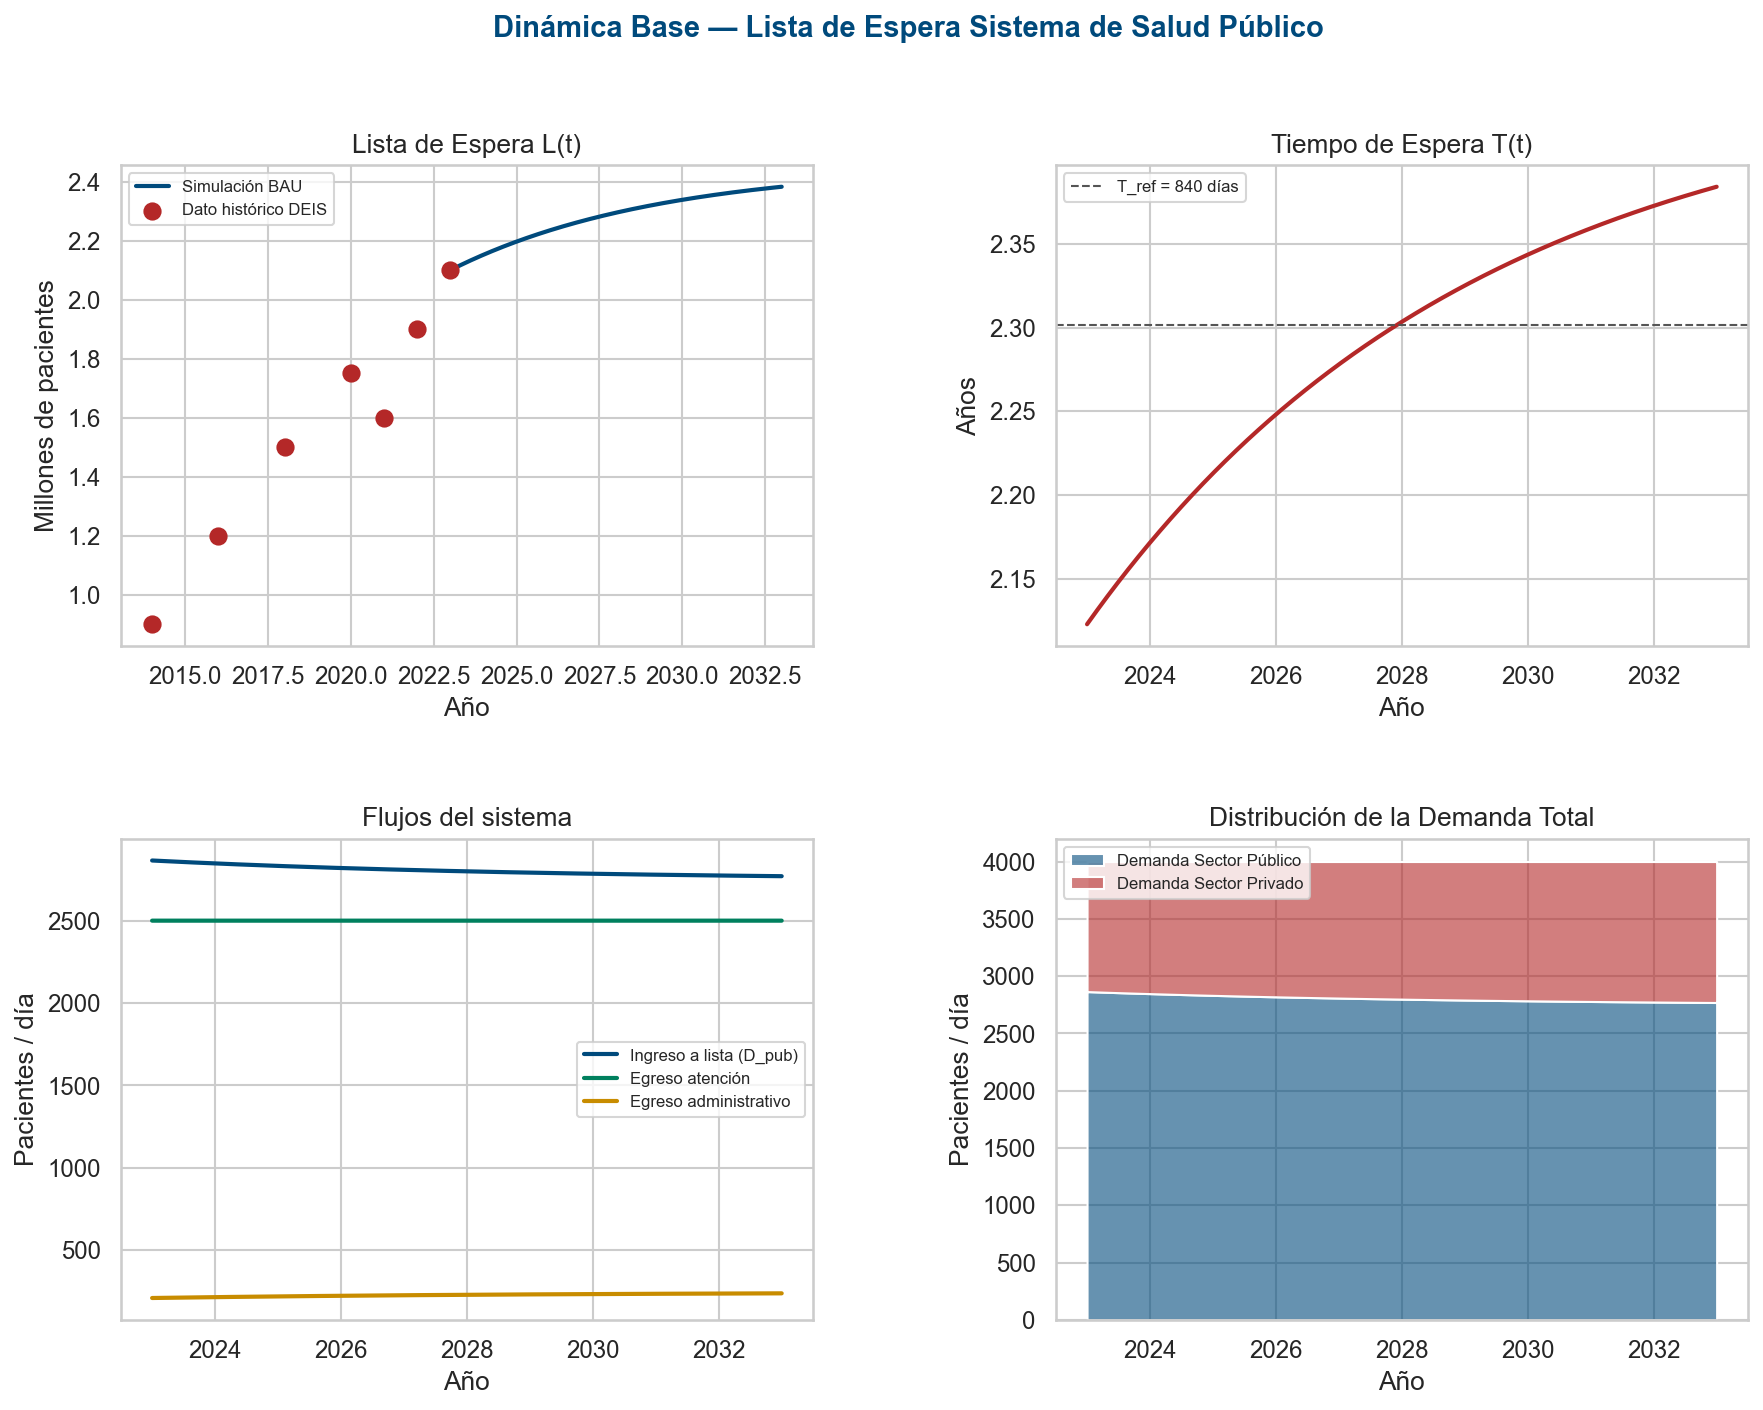
\includegraphics[width=1\linewidth]{fig1_dinamica_base.png}
    \caption{Dinámica del escenario base (modo normal): (a)~Lista de espera $L(t)$ con banda
  5--95\% y trayectoria histórica; (b)~Tiempo de espera (Ley de Little); (c)~flujos
  entrada/atención/fuga; (d)~erosión de capacidad (horas públicas y horas migradas
  acumuladas del bucle R1).}
    \label{fig:placeholder}
\end{figure}


\newpage
\subsection*{4.2 Escenarios de Política}

Se definen tres escenarios de política, cada uno alineado con una palanca distinta:

\begin{table}[H]
\centering
\caption{Definición de escenarios de política}
\label{tab:escenarios_def}
\begin{tabularx}{\textwidth}{@{}p{4.2cm}Xp{3.2cm}@{}}
\toprule
\rowcolor{azulDS!15}
\textbf{Escenario} & \textbf{Intervención} & \textbf{Parámetro} \\
\midrule
BASE (BAU) & Sin cambios & --- \\[3pt]
E1 — Capacidad & Sumar un especialista a la dotación de Cirugía General
  & $n_{\text{esp}} = 6$ \\[3pt]
E2 — Depuración & Depuración activa de la lista (revisión, duplicados, casos resueltos)
  & $g = 19$ pac/mes \\[3pt]
E3 — Retención & Retención de especialistas: mitigar el diferencial salarial que activa R1
  & $s_{\text{brecha}} = 0$ \\
\bottomrule
\end{tabularx}
\end{table}

\begin{table}[H]
\centering
\caption{Resultados de escenarios — modo normal (lista media jul-2025 y banda 5--95\%)}
\label{tab:escenarios_res}
\begin{tabular}{@{}lrr@{}}
\toprule
\rowcolor{azulDS!15}
\textbf{Escenario} & \textbf{Lista media} & \textbf{Banda 5--95\%} \\
\midrule
BASE (BAU)                 & 2006 & [1302, 2711] \\
E1 — Capacidad ($n=6$)     & \textbf{81}   & [6, 353] \\
E2 — Depuración ($g=19$)   & 1402 & [693, 2128] \\
E3 — Retención ($s_{\text{brecha}}=0$) & 1958 & [1278, 2653] \\
\bottomrule
\end{tabular}
\end{table}


\begin{figure}[H]
    \centering
    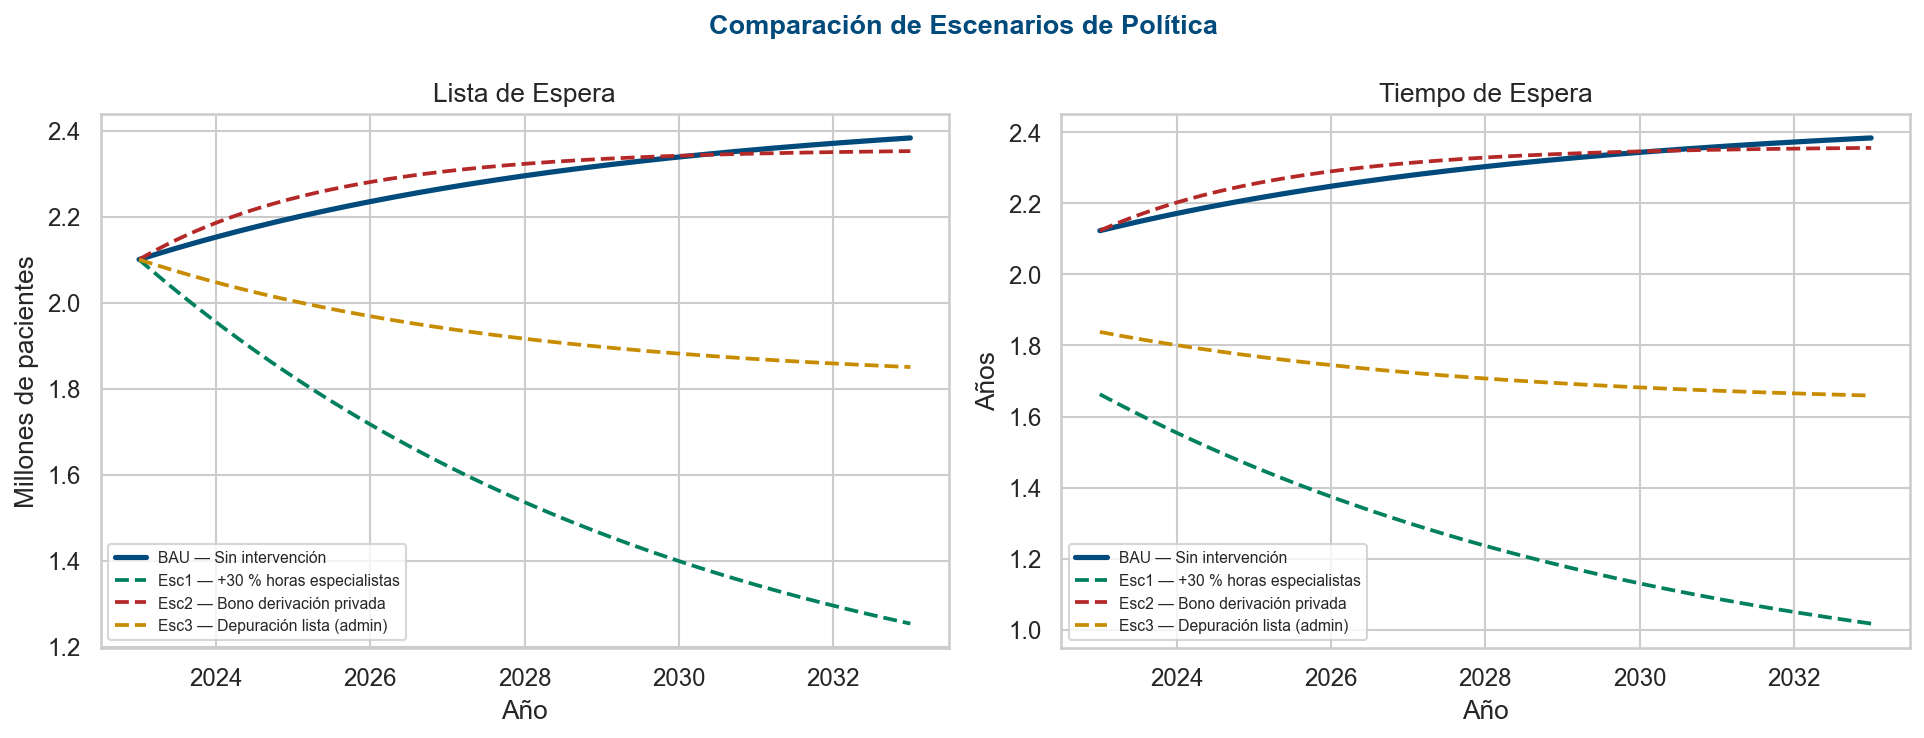
\includegraphics[width=1\linewidth]{fig3_escenarios.png}
    \caption{Comparación de escenarios de política (modo normal). \textbf{Izquierda:}
    lista de espera $L(t)$. \textbf{Derecha:} tiempo de espera. La intervención E1
    (capacidad) cambia cualitativamente el comportamiento del sistema.}
    \label{fig:placeholder}
\end{figure}

\subsection*{4.3 Efecto del Bucle R1 y el Tipping Point de Capacidad}

\subsubsection*{El bucle R1 es un amplificador de segundo orden}

Comparando el modelo con el bucle de erosión activado y desactivado en modo normal, la lista media de julio de 2025 pasa de 1958 (bucle OFF) a 2006 (bucle ON), un efecto de $+48$ pacientes. Bajo la calibración actual, el bucle R1 es un amplificador de segundo orden y no el motor principal del crecimiento. Esto es coherente con el escenario E3 ($s_{\text{brecha}}=0$): anular el bucle reduce la lista media solo de 2006 a 1958. El motor dominante del crecimiento es la brecha estructural entre capacidad y demanda, no la erosión salarial; pero el bucle R1 sigue siendo relevante a largo plazo por su irreversibilidad.

\subsubsection*{El sistema vive al filo del tipping point}

La sensibilidad a la capacidad (Tabla~\ref{tab:sens_cap}) muestra que entre 5 y 5.5 especialistas el sistema cruza un umbral: con 5 especialistas la lista crece a 2006, con 6 cae a 81. La razón es que la capacidad base ($\approx 240$ pac/mes) está estructuralmente por debajo de la demanda media ($\approx 275$ pac/mes) pero muy cerca de ella. El sistema vive al filo: pequeños cambios en la capacidad producen cambios cualitativos de comportamiento, el rasgo característico de un punto de inflexión.

\subsection*{4.4 Conclusión — Respuesta a la Pregunta de Investigación}

\textbf{¿Qué factores estructurales explican el crecimiento?}

El crecimiento persistente de la lista de Cirugía General se explica por un desequilibrio estructural entre flujos: la entrada media ($\approx 275$ pac/mes) supera de forma sostenida la capacidad de resolución pública ($\approx 240$ pac/mes con la dotación actual). La lista vive al filo de un punto de inflexión: la capacidad está estructuralmente por debajo de la demanda pero tan cerca que un solo especialista adicional revierte la tendencia. Los bucles balanceadores B1 (fuga al privado) y B2 (egreso administrativo) frenan el crecimiento pero no lo revierten; el bucle reforzador R1 (erosión salarial) lo amplifica de manera secundaria bajo la calibración actual.

\textbf{¿Qué política es más efectiva?}

De los tres escenarios, E1 (aumento de capacidad pública) es con diferencia el más eficaz: sumar un especialista reduce la lista media de 2006 a 81 pacientes, cruzando el tipping point. La capacidad es la palanca dominante. La depuración administrativa (E2) ayuda de manera apreciable y monótona (de 2006 a 1402), pero su efecto es proporcionalmente menor. La retención de especialistas (E3, mitigar el bucle salarial) tiene un efecto menor en esta calibración (de 2006 a 1958), pero es estructuralmente relevante a largo plazo porque el bucle R1 es irreversible: una vez que el especialista migra horas, no las recupera.

\textbf{Implicancia sistémica:} la palanca de mayor apalancamiento es elevar la capacidad pública, pues actúa directamente sobre el límite estructural del arquetipo \textit{Límites al Crecimiento}. La depuración es un complemento útil de corto plazo. La retención de especialistas, aunque de efecto modesto en el horizonte estudiado, protege la capacidad futura y debe sostenerse como política de largo plazo. No hay una única intervención suficiente, pero la jerarquía es clara: capacidad primero.

\newpage
% ============================================================
\section*{Referencias}
\addcontentsline{toc}{section}{Referencias}
% ============================================================

\begin{enumerate}[leftmargin=1.5cm,label=\textbf{[\arabic*]}]

\item \label{ref:sigte} \textbf{SIGTE-SSVSA — Sistema de Información para la Gestión de Tiempos de Espera}

\item \label{ref:cde} \textbf{Hospital Eduardo Pereira (CDE) — Operación del Servicio de Cirugía General}

\item \label{ref:nb} \textbf{Regresión Binomial Negativa de la fuga al privado}

\item \textbf{Barlas, Y. (1989).} Multiple tests for validation of system dynamics type of
  simulation models. \textit{European Journal of Operational Research}, 42(1), 59--87.

\item \textbf{Sterman, J.D. (2000).} \textit{Business Dynamics: Systems Thinking and Modeling
  for a Complex World.} McGraw-Hill.

\item \textbf{Meadows, D. (2008).} \textit{Thinking in Systems: A Primer.} Chelsea Green.

\item \textbf{Little, J.D.C. (1961).} A proof for the queuing formula: $L=\lambda W$.
  \textit{Operations Research}, 9(3), 383--387.

\item \textbf{González-Busto, B. \& García, R. (1999).} Waiting lists in Spanish public
  hospitals: a system dynamics approach. \textit{System Dynamics Review}, 15(3), 201--224.

\item \textbf{Wolstenholme, E.F. (1999).} A patient flow perspective of UK health services:
  exploring the case for new "intermediate care" initiatives.
  \textit{System Dynamics Review}, 15(3), 253--271.

\item \textbf{DEIS/MINSAL.} Estadísticas de salud (contexto general del sistema público chileno).\\
  \url{https://deis.minsal.cl/estadisticas-de-salud/}

\end{enumerate}

\end{document}
